\chapter{Oscilloscope}
 
 The PICSimLab has a basic two-channel oscilloscope that can be used to view the signal on any pin 
 of the microcontroller. The oscilloscope can be accessed through the ``Modules->Oscilloscope'' menu.
\begin{figure}[H]
\center
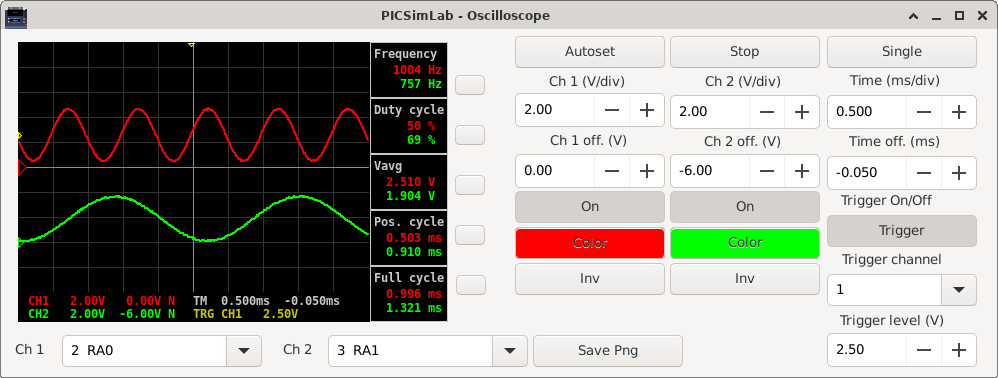
\includegraphics[width=0.99\textwidth]{img/osc.png} 
\end{figure} 

The oscilloscope supports up to 4 simultaneous measurements of the type: 
\begin{itemize}
 \item Vmax
 \item Vmin
 \item Vavg
 \item Vrms
 \item Frequency
 \item Duty cycle
 \item Pos. cycle
 \item Neg. cycle
 \item Full cycle
\end{itemize}


